\chapter{\textit{DE} híbrido para \textit{FJSSP}}
\section{Introducción}

El problema de JSSP (\textit{Job Shop Scheduling Problem}) es uno de los problemas más importantes y difíciles en el campo de la programación de tareas. El problema FJSSP (\textit{Flexible Job Shop Scheduling Problem}) es una extensión del JSSP clásico, en el que las operaciones pueden ser procesadas por cualquier máquina de un conjunto dado, en lugar de una máquina específica. En general, el FJSSP está mucho más cerca de un entorno de producción real y tiene una aplicabilidad más práctica. Sin embargo, el FJSSP es más complejo que el JSSP debido a su decisión adicional de asignar cada operación a la máquina apropiada además de las operaciones de secuenciación en las máquinas. Fue probado que FJSSP es NP-duro si cada trabajo tiene como mínimo tres operaciones y hay al menos dos máquinas \cite{Garey}.


Ante la búsqueda de soluciones a problemas de tan alta complejidad, en los últimos años el interés en las metaheurísticas híbridas ha aumentado considerablemente en el campo de la optimización. Los mejores resultados encontrados para muchos problemas de optimización clásicos o de la vida real se obtienen mediante algoritmos híbridos \cite{Talbi}. En este trabajo, será considerado un algoritmo de evolución diferencial híbrido para hacer frente al problema FJSSP planteado.


La resolución de un problema de optimización complejo y/o de alta dimensión puede beneficiarse de la distribución del computo. La idea es resolver pequeñas partes del problema y alcanzar la mejor solución en un tiempo razonable \cite{Apolloni}. Esta idea puede ser llevada al algoritmo que resuelve el problema de optimización.


En este capítulo será descrito el problema FJSSP a resolver, el diseño de la representación y evaluación de soluciones, la decodificación de soluciones, un algoritmo de búsqueda local, y por último la implementación de un algoritmo de \textit{DE} híbrido para el problema de \textit{FJSSP}. 

\section{FJSSP: \textit{Flexible Job Shop Scheduling Problem}}

En comparación con el JSSP (\textit{Job Shop Scheduling Problem}) clásico, donde se requiere que cada trabajo se procese en una sola máquina, la asignación de tareas en FJSSP es más desafiante, ya que requiere una selección adecuada de una máquina de un conjunto de máquinas determinadas para procesar cada operación. Eso significa que el FJSSP consta de dos subproblemas. El primero es asignar cada operación a una máquina de un conjunto de máquinas capaces, y el segundo trata de la secuenciación de las operaciones asignadas en todas las máquinas.


El problema puede ser descrito de la siguiente manera. Dado un conjunto de trabajos independientes \text{$J = \{J_1, J_2, . . . , J_n\}$}. Un trabajo $J_i$ está formado por una serie de operaciones $O_{i1},O_{i2}, . . . , O_{in_i}$ que se realizarán una después de la otra de acuerdo con la secuencia dada. El conjunto de máquinas $U = \{M_1,M_2, . . . , M_m\}$ es dado. Cada operación $O_{ij}$ puede ejecutarse en cualquiera de los subconjuntos $U_{ij} \subseteq U$ de máquinas compatibles. Se tiene flexibilidad parcial si existe un subconjunto adecuado $U_{ij} \subset U$ para al menos una operación $O_{ij}$, en cambio, se tiene flexibilidad total si $U_{ij} =U$ para cada operación $O_{ij}$. El tiempo de procesamiento de cada operación depende de la máquina, por lo tanto, $d_{ijk}$ es el tiempo de procesamiento de la operación $O_{ij}$ cuando se ejecuta en la máquina $M_k$. No se permite la anticipación, es decir, cada operación debe completarse sin interrupción una vez iniciada. Además, las máquinas no pueden realizar más de una operación a la vez. Todos los trabajos y máquinas están disponibles en tiempo 0.


El problema es asignar cada operación a una máquina apropiada (problema de enrutamiento) y secuenciar las operaciones en las máquinas (problema de secuenciación) con el fin de reducir el tiempo de terminación (\textit{makespan} en inglés). Esta medida es el tiempo necesario para completar todos los trabajos del problema y se define como $C_{max} =max_i\{C_i\}$, donde $C_i$ es el tiempo de finalización del trabajo $J_i$. La tabla \ref{tab:proccesingTime} muestra una instancia del problema FJSSP con 3 trabajos, 4 máquinas y 8 operaciones. Las filas y columnas corresponden, respectivamente, a operaciones y máquinas, y las entradas de la tabla son los tiempos de procesamiento requeridos. En este ejemplo, se tiene un escenario flexible parcial, una entrada de $\infty$ en la tabla significa que una máquina no puede ejecutar la operación correspondiente, es decir, no pertenece al subconjunto de máquinas compatibles para esa operación. Siguiendo el paradigma de los algoritmos evolutivos, llamaremos a cualquier solución del problema como un individuo o cromosoma.


% Table generated by Excel2LaTeX from sheet 'Hoja1'
 \begin{table}[!b]
    \scriptsize
   \centering
   \caption{Tabla de tiempo de procesamiento}
     \begin{tabular}{|c|c|c|c|c|c|}
    \hline
           & & $M_1$    & $M_2$    & $M_3$    & $M_4$ \\ \hline
     \multirow{$J_1$} & $O_{11}$   & $\infty$     & 6     & 5    & $\infty$ \\
     & $O_{12}$   & 4     & 8     & 5     & 6 \\
     & $O_{13}$   & 9     & 5     & $\infty$     & 7 \\\hline
     \multirow{$J_2$} & $O_{21}$   & 2     & $\infty$     & 1    & 3 \\
     & $O_{22}$   & 4     & 6     & 8     & 4 \\
     & $O_{23}$   & 9     & $\infty$     & 2     & 2 \\\hline
     \multirow{$J_3$} & $O_{31}$   & 8     & 6     & $\infty$     & 5 \\
     & $O_{32}$   & 3     & 5     & 8     & 3 \\ \hline
     \end{tabular}%
   \label{tab:proccesingTime}%
 \end{table}%

\section{Representación y evaluación de soluciones}

Un punto de diseño fundamental en el desarrollo de metaheurísticas es la codificación (representación de una solución) a utilizar. En este caso, se consideró la propuesta por Bierwirth en \cite{bierwirth1995} que es adecuada y relevante para el problema de optimización abordado, la cual se basa en una permutación con repeticiones. Una solución, $S$, es una permutación del conjunto de operaciones que representa un pedido tentativo para ordenar su programación, cada una representada por su número de trabajo. Por ejemplo, dado el vector $x_i^g=[0.6,-0.5,0.4,-0.3,-0.1,0.9,-0.7,0.2]$, este será convertido a $[2, 1, 1, 3, 2, 2, 1, 3]$. Tal como se observa, el largo del vector $x_i^g$ es equivalente a la cantidad de operaciones. Esta programación válida se corresponde con la secuencia de operaciones $S=[O_{21}, O_{11}, O_{12}, O_{31}, O_{22}, O_{23}, O_{13}, O_{32}]$. 


Otro punto de diseño común es la definición de la función objetivo que guiará la búsqueda hacia soluciones "buenas" dentro del espacio de búsqueda. Al evaluar $S$, el valor objetivo es el tiempo de terminación de esta solución. Para calcular este valor, cada operación $O_{ij}$ en $S$ se asigna a una máquina viable $M_k$ en el subconjunto $U_{ij}$ con el tiempo de finalización más corto, y luego se actualiza la carga de $M_k$. Como solución inicial se utiliza un procedimiento aleatorio, principalmente porque no se conocen heurísticas de construcción de alto rendimiento para FJSSP.


\section{Decodificación de soluciones}
En este trabajo, para mantener la simplicidad y las propiedades de DE en su configuración natural el algoritmo DE manipula vectores con valores reales. Consecuentemente, la decodificación de las soluciones consiste en convertir un vector de reales $x = (x_{1}, x_{2}, . . . , x_{D}) \in \mathbb{R}^{D}$ a la codificación propuesta por Bierwirth, descripta en la sección anterior, para obtener una solución $S$.


Para realizar esta conversión, la regla del valor de posición más grande (\textit{largest position value} o LPV en inglés) presentada en \cite{YuanYuan} se emplea primero para construir una permutación de operaciones sin repeticiones al ordenar los valores del vector de reales en forma decreciente en conjunto con el vector de posiciones. Luego, se transforma el vector de permutaciones sin repeticiones al esquema de vector de permutaciones con repeticiones (solución) propuesto por Bierwirth. Para esto se itera sobre el conjunto $J = \{J_1, J_2, . . . , J_n\}$ de trabajos y dentro sobre cada posición del vector de permutaciones, si la operación contenida en la posición tratada pertenece al trabajo $J_i$, se cambia el valor de $S[j]$ por el de $J_i$. En el algoritmo \ref{alg:algoritmoDecodificacion} se puede apreciar la especificación del proceso realizado.

\begin{algorithm}[!tb]
    \caption{Pseudocódigo del algoritmo de decodificación de soluciones} \label{alg:algoritmoDecodificacion}
    \begin{algorithmic} [1]
    \Require {$x = (x_{1}, x_{2}, . . . , x_{D})$} 
    \Ensure {$S[D]$} 
        \State $S[D] \leftarrow $ LPV($x$)
        \For {cada vector $J_i$ de $\{J_1, J_2, . . . , J_n\}$}
            \For {cada posición $j$ de $S[D]$}
                \If{$S[j]$ es una operación de $J_i$}
                    \State $S[j] \leftarrow  J_i$
                \EndIf
            \EndFor
        \EndFor
    \end{algorithmic}
\end{algorithm}

En la Figura \ref{fig:decodificacion} se puede ver un ejemplo de este procedimiento para una instancia del problema FJSSP con 3 trabajos, 4 máquinas y 8 operaciones mostrada en la Tabla \ref{tab:proccesingTime}.

\begin{figure}[h]
    \centering
    \includegraphics[width=0.8\textwidth]{images/Decodificacion.eps}
    \caption{Ejemplo del proceso de decodificación de una solución para una instancia del problema de FJSSP.}
    \label{fig:decodificacion}
\end{figure}

\section{DE y búsqueda local}

Con el fin de mejorar la eficiencia de DE al resolver el FJSSP, se incorporó al algoritmo un procedimiento de búsqueda local simple, en el que se se seleccionan e intercambian al azar dos posiciones del vector de prueba. Si hay una mejora en la función objetivo, se acepta el intercambio, de lo contrario, no se considera. En el Algoritmo \ref{alg:algoritmoLS} se puede ver un pseudocódigo del procedimiento de búsqueda local.


Este procedimiento de búsqueda local se aplica a los vectores de prueba de la próxima generación (justo antes de la línea 10 del Algoritmo \ref{alg:algoritmoDE}), lo que es beneficioso para evitar quedar atrapado en un óptimo local. Una característica importante de este procedimiento de búsqueda local es que no necesita una conversión hacia atrás, es decir, se aplica directamente sobre el vector de prueba. 


La frecuencia de búsqueda local está controlada por la probabilidad $P_{BL}$. La búsqueda local se puede aplicar a cada individuo de la población o a solo unos pocos. Aplicar una búsqueda local a cada individuo de la población puede desperdiciar recursos sin proporcionar más información útil que hacerlo solo a una pequeña fracción de la población. El uso de una gran fracción de la población puede limitar la exploración del espacio de búsqueda al permitir que el algoritmo genético evolucione durante un pequeño número de generaciones. Un uso más selectivo de la búsqueda local puede mejorar la eficiencia de los híbridos. La probabilidad de búsqueda local puede afectar la velocidad de convergencia del algoritmo. Este efecto no debe ignorarse al decidir entre diferentes probabilidades de búsqueda local.


\begin{algorithm} [H]
    \caption{Pseudocódigo de la Búsqueda local} \label{alg:algoritmoLS} 
    \begin{algorithmic} [1]
        \For {cada vector $x_{i}$ de $P$}
            \If {$random() < P_{BL}$} %\Comment $P_{BL}$: probabilidad de búsqueda local
                \State $j$ , $k \leftarrow $ random(1,$D$)
                \State $u_{i} \leftarrow $ intercambiar($x_{i}$, $j$,$k$)
                \If {$f(u_{i}) \leq  f(x_{i})$} \Comment{para un problema de minimización}
                    \State $x_{i} \leftarrow u_{i}$
                \EndIf
            \EndIf
        \EndFor
    \end{algorithmic}
\end{algorithm}




\section{\textit{DE} y paralelismo} \label{subsec:DEparalelo}

Actuando sobre la eficiencia del algoritmo, se incorporó un paralelismo a nivel de iteración, con el fin de acelerar el algoritmo reduciendo el tiempo de búsqueda. Como \textit{DE} es una metaheurística basada en población se consideró un esquema de maestro-trabajador, donde los trabajadores realizan las operaciones de mutación, recombinación y evaluación de la función objetivo, y el maestro al recibir de los trabajadores las soluciones ya evaluadas, realiza el proceso de selección. En la figura 
\ref{fig:ParalelizacionDE} se puede observar cómo se realiza la paralelización para 4 CPUs.


Para la búsqueda local también se implementó un paralelismo a nivel de iteración, como se puede observar en la figura \ref{fig:ParalelizacionLS}, donde los distintos vecinos son divididos en diferentes particiones del mismo tamaño. Una vez generadas las particiones, se aplica la búsqueda local a cada uno de sus individuos y luego se evalúan. Las operaciones en las particiones ocurren en forma paralela e independiente. Este esquema otorga grandes ventajas en cuanto a velocidad y aprovechamiento de recursos. 


\begin{figure}[h]
    \centering
    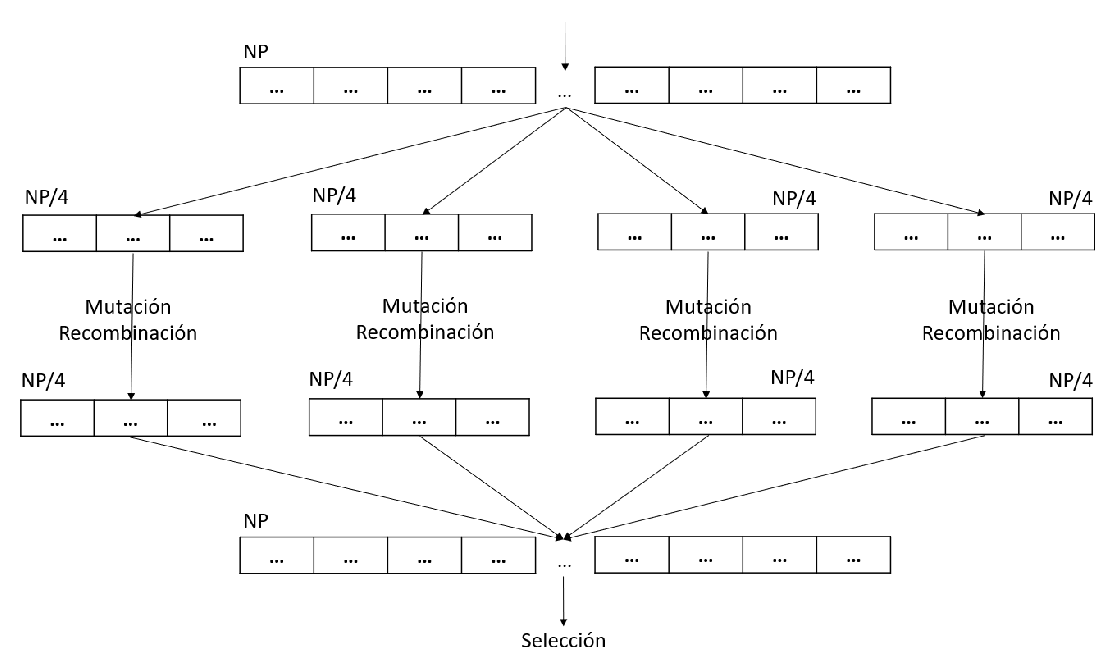
\includegraphics[width=\textwidth]{images/Paralelizacion-DE.eps}
    \caption{Paralelización del algoritmo DE.}
    \label{fig:ParalelizacionDE}
\end{figure}

\begin{figure}[H]
    \centering
    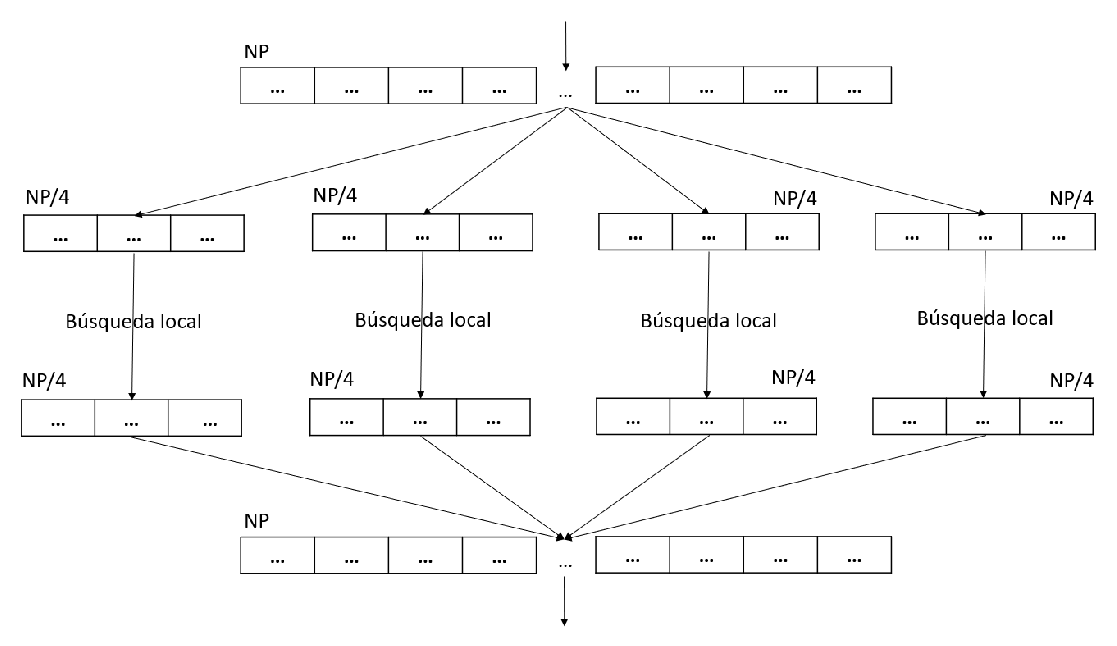
\includegraphics[width=\textwidth]{images/Paralelizacion-LS.eps}
    \caption{Paralelización de la búsqueda local.}
    \label{fig:ParalelizacionLS}
\end{figure}

\section{\textit{HDE} para el \textit{FJSSP}}
El algoritmo \ref{alg:algoritmoDEhibrido} presenta el pseudocódigo del algoritmo de \textit{DE} híbrido para \textit{FJSSP}. Como se puede observar el esquema general es el mismo que el presentado en el capítulo anterior, con la inclusión del proceso de búsqueda local. Además, se agrega como entrada la probabilidad de aplicar búsqueda local ($P_{BL}$), con el fin de permitir al investigador realizar cambios sobre el parámetro.

\begin{algorithm} [H]
    \caption{Pseudocódigo de la Evolución Diferencial (DE)} \label{alg:algoritmoDEhibrido}
    \begin{algorithmic} [1]
    \Require {$F, Cr, N_p, P_{BL}$} 
    \Ensure {$x_{best}$} 
        \State inicializar($P$,$N_p$) 
        \State $g \leftarrow 0$
        \While {no se alcance la condición de fin}
            \For {cada vector $x_{i}^g$ de $P^g$}
                \State $v_{i}^g \leftarrow $ mutación($x_{i}^g, P^g, F$) 
                \State $u_{i}^g \leftarrow $ recombinación($x_{i}^g, v_{i}^g, Cr$)
                \State $x_{i}^{g+1} \leftarrow $ selección($x_{i}^g, u_{i}^g$)
                \State agregar($P^{g+1}, x_{i}^{g+1}$) 
            \EndFor
            \State búsqueda-local($P^g$, $P_{BL}$)
            \State $g \leftarrow g+1$ 
        \EndWhile
        \State$x_{best} \leftarrow $mejor-solución($P^{g}$)

    \end{algorithmic}
\end{algorithm}